%%background
This chapter presents a detailed discussion of the important theoretical concepts on the subject to provide an understanding of the project 
undertaken. 

\section{Internet Scanning}
Internet Scanning is the process of using network scanning techniques to conduct scans on a large scale. Network Scanning is defined 
as the process of identifying hosts on a network by using features in the network protocol to ping devices or hosts and of analysing 
information based on the data received by those pings. The basic concept of network scanning is to identify all hosts connected to a network and map them
to their IP addresses. This process is achieved by sending packets to addresses and in turn discover what is on the network based on the data received. 
All the active hosts in the network will respond to this ping while the inactive hosts will have no response. The feedback from this scan 
gives information about how the hosts behave with internal and external components of a network. Another technique called ``Port Scanning'' 
can be used to gather information about open ports that can receive or send information for the identified hosts in the network.\\ 
Performing network scans can have both good and bad implications. While some entities use network and port scanning to identify weaknesses, 
some may use it to exploit the weakness in the network to gain access to information they are not privy to~\cite{mou21}. 
\newpage

\subsection{MaxMind Geolocation IP Databases and Services}
Maxmind provides services packaged in APIs and databases that provide accurate IP intelligence data. The web services give the most 
accurate IP geolocation data and can be accessed through APIs in almost every programming language. The GeoIP2 databases provide in-depth information
for IPv4 network blocks and are locally maintained for high volume, fast lookup purposes and allow unlimited use. Since the GeoIP2 databases
are now commercial, the project uses the free version called GeoLite2 databases that are slightly less accurate than the former and are 
updated weekly. The databases include information about the entire IPv4 address space for all countries. These APIs and databases are 
used for a variety of purposes like detecting network vulnerabilities and fraud detections~\cite{GeoLite265:online}. 
The program for this project required a dataset containing IPv4 addresses and their associated country name and country codes. Multiple Maxmind 
datasets were used to gather this information, and Python was used to generate the dataset required by combining information from different datasets. 
To get access to Maxmind, an account was made through their website in order to obtain the license key required to use the services mentioned above. 

\subsection{ZMap and ZGrab}
ZMap is an open-source fast single packet network scanner that is capable of scanning the entire IPv4 address space in under 45 minutes 
from a single standard machine. It provides the user with various probe modules including TCP SYN scans, ICMP, DNS queries, UPnP BACNET and can also send UDP probes.
Compared to other tools in the market ZMap achieves a better performance due to its architecture which is optimised for carrying out 
internet-wide surveys~\cite{182948}. This project makes use of the SYN module for identifying open ports. A TCP SYN scan involves the sending of an 
SYN packet to open a connection with a host on a specific port. If there is an SYN/ACK response from the host that indicates there is an open TCP/IP port. 
In case there is an RST response instead of an ACK, that indicates the particular port is closed~\cite{SYN}.

\noindent ZGrab is ZMap's sister project and an open-source fast application-layer network scanner designed to perform extensive internet-wide surveys. 
It works in combination with ZMap, but can also be used independently. It provides detailed information about the network handshakes and captures 
most of the meta-data during a TLS negotiation like the TLS certificates and banner information. It is built using Golang and is capable of carrying 
out the scanning process for all standard protocols like HTTP, SSH, IMAP and more. It provides the output in JSON format for each IP scanned for 
the selected protocol~\cite{zgrab2Github}.
\pagebreak

\subsection{Ethical Considerations}   
As stated above, network and port scanning techniques are carried out for various purposes. While network 
administrators or academics use these techniques to identify vulnerabilities or weaknesses, cyber attackers can use the same techniques to 
gain access to systems they are not privy to. Since the project requires carrying out active scans to understand the extent of public key reuse, it is 
important to consider whether there are any ethical implications for the hosts we are scanning. To carry out the scanning process, 
Durmeric et al. \cite{182948} have summarised some best practices one needs to consider as it is next to impossible to get permissions in advance 
from all hosts that are being scanned and assessed. Some of these practices include:
\begin{itemize}
    \item Ensuring scans will not overwhelm the network.
    \item Providing the nature of the scans in the form of webpages and DNS entries.
    \item Having a clear scope of the project and explaining the purposes of the scans.
    \item Limiting scanning when possible.
    \item Having a simple opt-out method.
\end{itemize}

\noindent In considering the points mentioned above, Dr.~Farrell carried out these scans using his Virtual Private Server and had a DNS TXT record 
that indicated the nature of the scans. Also, the project scans hosts that are mail servers, and hence, it is less likely to come across 
sensitive information since individuals do not run most mail servers. The scan rate for the ZMap and ZGrab tools was limited to not cause any 
disruptions to the active services in the network. The default blocklists that were used and provided by the ZMap included: local, reserved, and multicast IPv4 addresses.\\
Another factor that was considered besides the ones stated above was the secure storage and reporting of the data collected. All data 
was securely stored locally on my machine, and the analysis was also carried out on the same machine to report the key reuse scenarios. 
All IP addresses were anonymised in this report, and no domain names were released.

\section{Public Key Infrastructure} 
The Public Key Infrastructure (PKI) is a framework that comprises of set of policies, guidelines, and technologies that different enterprises, 
vendors and other entities can use to establish and maintain authentication and confidentiality while communicating over the internet. 
The PKI works on the core concept of public-key cryptography or known as asymmetric encryption. It comprises of a public and private key 
or more commonly referred to as a key-pair. 
Consider, for example, Bob wants to send a message to Alice securely. Both of them have knowledge about their respective key-pair. The following 
figure demonstrates how Bob would send a message to Alice using asymmetric encryption. 

\begin{figure}[h!]
    \centering
    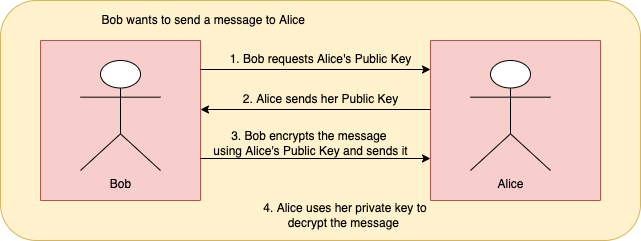
\includegraphics[width=15cm]{asym_encrp.png}
    \caption{Asymetric Encryption}
\end{figure}

\noindent A key over here is defined as a randomly generated sequence of bits. The public and private keys are closely related by 
some mathematical operations. But the question that arises here is how Bob knows that it was Alice who sent her public key. 
How can Bob authenticate the identity of Alice? This is where Digital Certificates play a crucial role, as they help in associating a public key 
with a person or an entity that allows authentication. These certificates are issued by Certification Authorities or commonly known as CAs. They are usually a third-party 
organisation (Eg: Digicert) responsible for issuing, revoking, and distributing certificates. The CA is trusted by all parties involved in 
the PKI, which would be Bob and Alice.

\noindent Now Bob can ask the CA for Alice's certificate, which contains information about Alice's public key. Since Bob trusts the CA and 
the CA is vouching for Alice, Alice's identity could be authenticated.\\
The PKI is deployed in a variety of environments over the internet to secure them, and some instances are web browsers, emails, 
file security etc~\cite{PublicKe39:online}. 

\section{Transport Layer Security}
Transport Layer Security (TLS) is a cryptographic protocol used to transfer data between applications over the internet securely. In today's day and age, 
TLS is one of the widely adopted protocols as it is majorly used in web browsers to ensure a secure session has been established. It can also be used for the safe 
transfer of data for different applications such as email, file transfers, voice-over-IP, and DNS. TLS does not secure data on the end systems but is used to 
facilitate secure data transfer from one point to another over the internet. As a result, no attacker can tamper or eavesdrop while the data is in transit. 
It is usually implemented over protocols like TCP/IP or UDP layer to secure application layer protocols like HTTP, IMAP, POP3, SMTP, and more. 
TLS was built on the Secure Socket Layer (SSL) protocol and was designed to be its replacement. It is a multilayered protocol that consists of:
\begin{itemize}
    \item \textbf{Handshake Protocol:} Authenticates the parties involved and negotiates an encryption algorithm and other parameters.
    \item \textbf{Record Protocol:} Ensures data is not tampered with when in transit using parameters negotiated during the handshake protocol.
\end{itemize}

\begin{figure}[h]
    \centering
    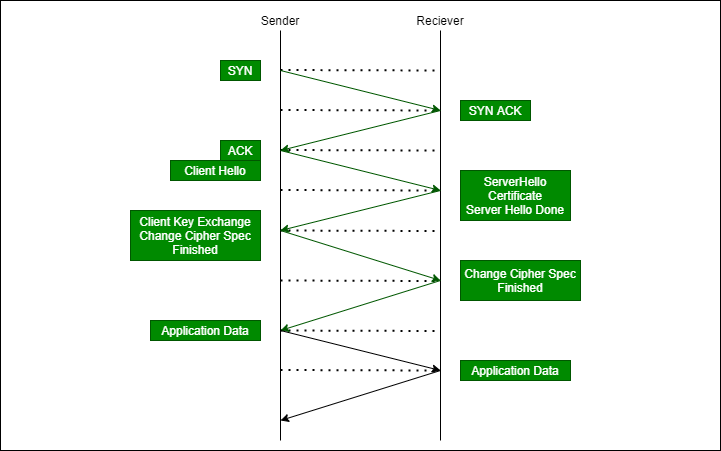
\includegraphics[width=14cm]{tls_hs.png}
    \caption{TLS Handshake Process}~\cite{Transpor60:online}
    \label{fig: TLS}
\end{figure}

\noindent Since the inception of TLS, it has been deployed in most of the web services on the internet because it protects sensitive information such as passwords, card details, emails, online chats,
browsing habits, etc. Since most websites work on a client-server model deploying TLS between the two endpoints protects sensitive information from attackers. TLS also makes use of the technique
of asymmetric cryptography which involves a key pair. In this scenario, the public key is used to encrypt the data by the sender and the receiver uses their private key to decrypt the data~\cite{rfc8446}.

\subsection{Implicit TLS v/s Opportunistic TLS}
Around the time when TLS was invented, plain text protocols like SMTP, POP3, and IMAP were already deployed heavily over the internet.
While many services supported the usage of the \textit{STARTTLS} command to upgrade the connection on the plain text ports, if a client 
did not support the same information would be transmitted in plain text before encryption was standardised. \textit{STARTTLS} or Opportunistic TLS was used 
to upgrade plain text connections to a secure one. Here the connection is upgraded after establishing the initial connection.\\
To normalise encryption over plain text protocols, new ports were decided upon by IANA. The difference here was that a TLS connection was immediately negotiated between 
the server and the client. If a server or client did not support TLS and the connection was not established, no information would be exchanged between 
the two. This is known as Implicit TLS. The use of Implicit TLS is preferred over the former to encourage consistency in 
how TLS is used~\cite{rfc8314}. The table below shows the ports used for each protocol using Implicit or Opportunistic TLS as decided upon 
by IANA~\cite{rfc6335}.
\begin{table}[h!]
    \centering
    \begin{tabular}{|c|c|c|c|c|}
        \hline
        Protocol &  Standard Port - No encryption & Implicit TLS Port & Opportunistic TLS Port\\
        \hline
        SMTP  &   25    &   587 &   25\\ 
        \hline
        POP3  &   110   &   995 &   110\\
        \hline
        IMAP &   143    &   993 &   143\\  
        \hline
        HTTP    &   80  &   443 &   -\\
        \hline
    \end{tabular}
    \caption{Implicit TLS vs Opportunistic TLS Ports}
    \label{tab:TLSports}
\end{table}

\subsection{TLS Certificates}
TLS certificates verify the ownership of a public key and are essential to secure connections and transactions over the internet. 
They are usually issued by some Certification Authority (CA) by signing the certificates indicating that the CA has verified the ownership. 
Whenever a user tries to connect to a server, the server sends them a certificate, and then the user verifies the server's certificate using the CA certificate 
present on the user's machine to establish a TLS connection. The certificates usually contain the following fields of information~\cite{rfc5280}:
\begin{itemize}
    \item Subject Domain Name
    \item Subject Organisation
    \item Issuing CA
    \item Alternative Subject Name 
    \item Date of Issue 
    \item Expiry Date 
    \item Public Key 
    \item Digital Signature by the issuing CA
\end{itemize}

\subsection{TLS Cipher Suites}
A cipher suite is defined as a set of cryptographic algorithms that are used by TLS to encrypt the information. It provides crucial 
information about securing data when using different network protocols like SMTP, HTTPS, POP3, etc. A cipher will dictate what algorithm is 
best suitable to make a secure and reliable connection to the server. A cipher suits provides the following information to a server:
\begin{itemize}
    \item \textbf{Key Exchange Algorithm:} Data over the internet is encrypted using a key. This provides the client and server with which algorithm to use for encryption/decryption of data.
    \item \textbf{Authentication Algorithm:} The server needs to verify the client's identity before sending or receiving any data. This field specifies that algorithm.
    \item \textbf{Bulk Data Encryption:} This is to ensure the secure transfer of data. 
    \item \textbf{Message Authentication Code Algorithm:} A MAC algorithm is sent along the with data to verify the contents of the data. 
\end{itemize}

\begin{figure}[h!]
    \centering
    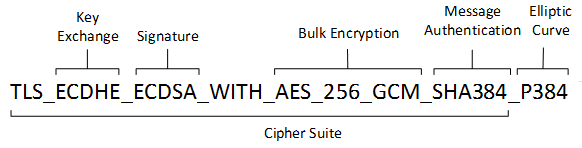
\includegraphics[width=10cm]{tls-cipher-suite.png}
    \caption{TLS Cipher Suite}~\cite{CipherSu69:online}
    \label{fig: CipherSuites}
\end{figure}

\subsection{Fingerprint SHA-256}
The concept of a key pair was introduced above. A fingerprint is defined as a short sequence of bytes used to identify a longer public key and is generated
by applying a hash function on a public key. SHA stands for Secure Hash Algorithm, which is used to shorten data into a minor sequence. The resulting 
output cannot be cracked unless a brute force attack is used, and this is where hashing differs from encryption. SHA256 is a popular cryptographic
algorithm that, if applied to a number consisting ``n'' bits, will return a 256-bit value. It is widely used in digital certificates and signatures. 

\section{Application Layer Protocols}
This section describes the ports we scan and the protocols associated with the ports. 
\begin{table}[h!]
    \centering
    \begin{tabular}{|c|c|c|}
        \hline
        Port &  Protocol\\
        \hline
        22  &   SSH\\ 
        \hline
        25  &   SMTP\\
        \hline
        110 &   POP3\\  
        \hline
        143 &   IMAP\\  
        \hline
        443 &   HTTPS\\ 
        \hline
        587 &   SMTP Submit\\  
        \hline
        993 &   IMAPS\\ 
        \hline
    \end{tabular}
    \caption{Ports Scanned}
    \label{table:alports}
\end{table}

\subsection{Secure Shell Protocol}
The Secure Shell (SSH) is a network communications protocol that enables two computers to communicate and share data remotely. 
Communication between the two machines is encrypted, meaning this protocol can be used over an insecure network to make it secure.
SSH consists of three layers: 
\begin{itemize}
    \item \textbf{Transport Layer:} Establishes safe connections between the server and the client for communications after the authentication process has been validated. Oversees data encryption, decryption, and integrity and provides caching and compression if needed. 
    \item \textbf{Authentication layer:} Conducts the authentication process, i.e.\ verifies the identity of the user.
    \item \textbf{Connection Layer:} Manages the communication between the two machines once authentication is completed and handles the opening and closing of each session. 
\end{itemize}

\noindent SSH requires a login from the user to start performing operations on the remote machine and can be used for the safe transfer of data. 
It works on a client-server model, i.e.\ the client will initiate the process by pinging the server, and in turn, the server responds to the client prompting them 
to finish the authentication process. The SSH server listens on some TCP/IP ports designated for SSH, and usually, TCP/IP port 22 is reserved for SSH servers.
Clients contact the server on this port to start the connection process~\cite{rfc4254}.

\begin{figure}[h!]
    \centering
    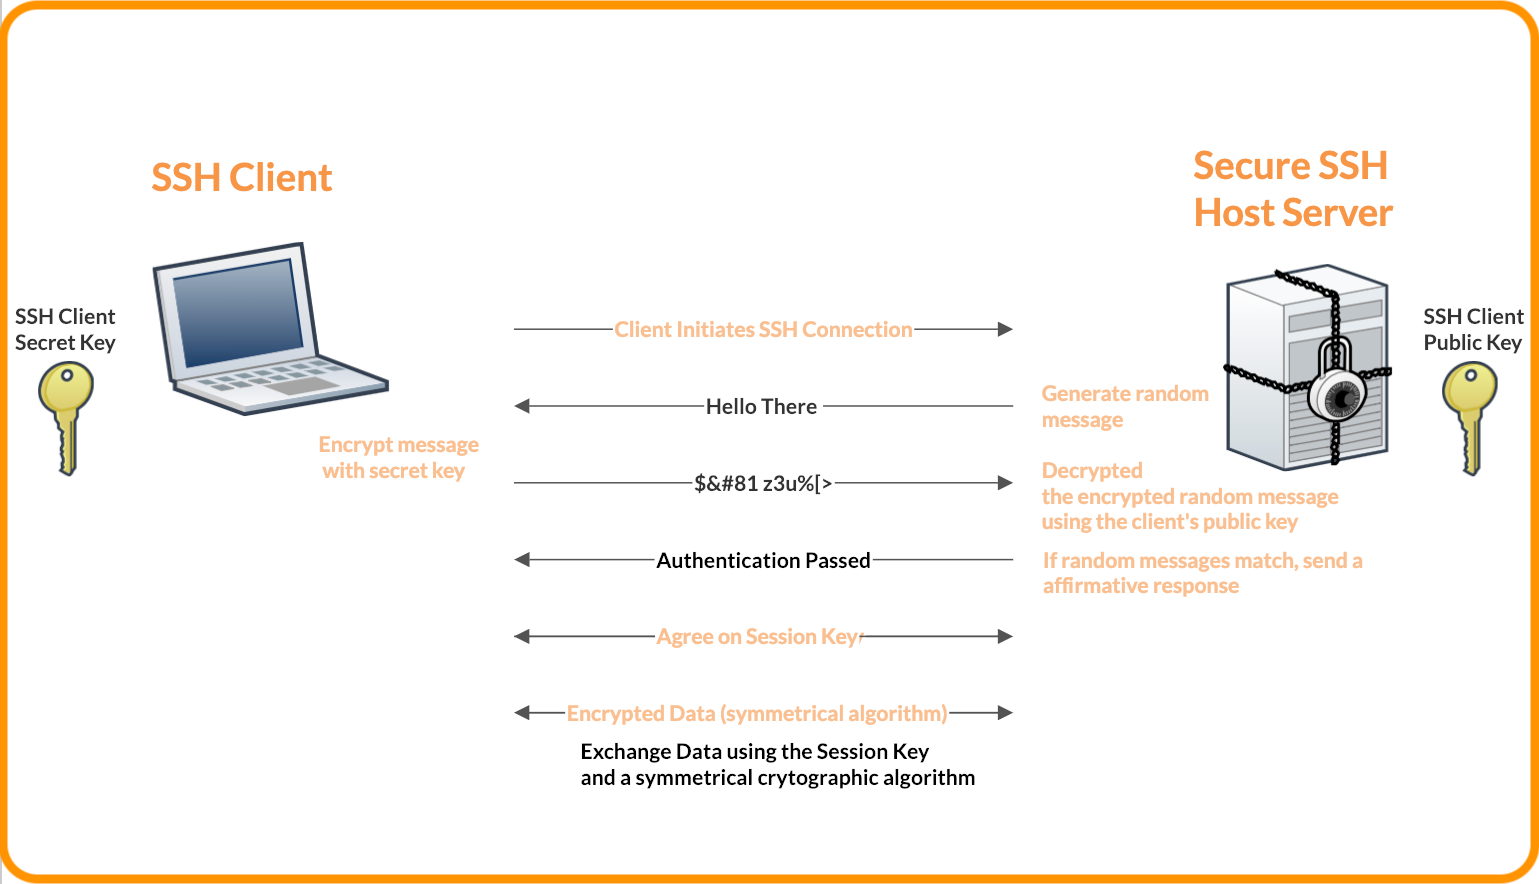
\includegraphics[width=13cm]{ssh_working.png}
    \caption{SSH Process}~\cite{LearnSSH25:online}
    \label{fig: SSHworking}
\end{figure}

\noindent SSH uses asymmetric cryptography similar to the PKI for the authentication process between the client and the server and uses symmetric encryption and other hashing algorithms
to encrypt the data transfer between the client and the server, ensuring privacy and integrity. Each SSH server should have at least one host key to ensure 
that the client communicates with the correct server during the key exchange. Ideally, each host should have a unique key, as key sharing between hosts can leave the host 
susceptible to man-in-the-middle attacks. However, key sharing may be acceptable and even practical (for instance, multiple hosts sharing keys but all under one entity). The Secure Shell Protocol is widely adopted and used for various purposes by individuals and Corporations. 
Some use cases are remote access to machines, port forwarding, virtual private networks, and many more.  

\subsection{SMTP/ (S)}
Simple Mail Transfer Protocol is used to transfer mail reliably and efficiently. A two-way connection is established with an SMTP server when an SMTP client wants to transmit a message. The main objective of this protocol is to transfer mail messages to an SMTP server 
or to report failure to incase it fails to do so. Traditional SMTP operates over assigned port 25 and usually does not provide encryption, meaning that the client and server communicate over the internet in plain text~\cite{rfc5321}. This can be considered a significant flaw as 
all communications are susceptible to eavesdropping or man-in-the-middle attacks while emails are in transit. 
SMTP over TLS or SMTPS was introduced to encrypt these communications. By using SMTP over TLS, one is wrapping SMTP commands inside 
a TLS connection. Usually, port 587 is used for SMTPS compared to port 25 for SMTP to distinguish between the two.

\noindent With the use of SMTP over TLS, the client waits for the \textit{STARTTLS} keyword from the SMTP server. After that, the TLS handshake 
protocol is completed. After the handshake is completed, the client and the server decide whether to continue ahead with the session based 
on the current privacy achieved. Some client-servers might choose to continue ahead even if no TLS authentication was attained, as traditionally 
SMTP operates without any encryption, while others may only decide to continue with the session based on specific authentication and 
privacy achieved..~\cite{rfc2487}.

\subsection{POP3 / (S)}
Post Office Protocol Version 3 or POP3 is a standard mail protocol used by mail servers and their clients to receive emails from a remote 
server and send it to a local client. It is a client-server protocol in which email is received and stored on a mail server, and a recipient of an email client 
can download emails from that server which enables the client to view the email offline. POP3 is embedded into most email clients. Once the 
email is on the client, POP3 can be configured to delete the email from the server or save the email for a specific period, allowing 
clients to download the mail as many times. The standard port assigned to POP3 is port 110, but usually, communication is over 
plain text on this port, but a secure connection can be established using the \textit{STARTTLS} command on this port. In case the client wants to 
connect securely, POP3 over TLS is used that is assigned to port 995~\cite{rfc1939}.

\subsection{IMAP/ (S)}
The Internet Message Protocol or IMAP is a standard mail retrieval protocol used to download mail messages by email clients. It enables 
users with control over mail boxes and enables with to organise them as per requirements. The port assigned to the IMAP protocol is 143, 
but it does not support encryption over that port. To secure it the \textit{``STARTTLS''} command can be used. Alternatively, port 993 can be used 
that supports IMAP or TLS (IMAPS) that establishes a TLS connection immediately.~\cite{rfc9051}.

\subsection{HTTPS}
HTTPS or HTTP over TLS is an alternative to simple HTTP over TCP. The difference here is that the HTTP client should also act as a TLS 
client. The client should initiate the connection, but before making an HTTP request, it should establish a TLS session by initiating the 
TLS handshake protocol. Once the handshake is completed, the client can start making HTTP requests to the server. All data exchanged between 
the client and the server is sent as TLS application data. To distinguish between HTTP over TCP and HTTP over TLS, both protocols have been 
assigned different port numbers. HTTP operates over port 80 while HTTPS operates over port 443~\cite{rfc2818}.

\section{Technology Evolution}
The development of the surveying program was previously done in 2017/18 using Python2. However, Python3 has gained popularity and has been 
widely adopted by corporations, individuals, and others. There are few notable differences between the two, and specific Python3 versions 
provide better performance than Python2 versions. Since January 1, 2020, support for Python2 has been discontinued. That means there
will be no further improvements for Python2 even if a significant bug or security flaw is found~\cite{10.5555/1593511}. Popular libraries 
like Pandas, NumPy, and many more have officially stopped supporting Python2 versions, which makes it even more critical to migrate the current code to 
Python3~\cite{Installa51:online}.\\
The previous program used ZGrab1 to run the scans back in 2017/18, and since then, ZGrab2 has been released, which has depreciated the last version. 
It contains a revamped framework that has simplified the tools' usage and allows individuals to add custom protocols over various ports by building them on their own using Golang. It has 
integration tests available which can help the development process and can be efficiently run using Docker~\cite{merkel2014docker,zgrab2Github}.\\
There were also some minor changes to how Maxmind ships the data needed for the program to work. Additional scripts and modifications to current ones were carried out to get 
the countrywide IP data to carry out the scans.

\newpage
\section{Code Refactoring}
\label{refactortechs}
Code refactoring can be defined as the restructuring of code to improve code readability, reduce complexity, and improve the 
maintainability and efficiency of the program. The refactoring process should contribute to the above factors, 
but the program's functionality should not be compromised. Refactoring enables developers to gain an in-depth understanding of 
the program and enables them to expand the program quickly by integrating more features efficiently and reducing the amount 
of technical debt.

\noindent Technical debt, also known as code debt, refers to when development is rushed or when code delivery is prioritised over 
writing quality code. To ensure code refactoring has yielded benefits, one needs to define a few metrics like \textit{``\% of duplicate code''} \cite{ThePower10:online}. 
Techniques like unit testing and functionality tests need to be performed regularly in order to ensure the refactoring process is beneficial~\cite{TheCompl71:online}. 
Refactoring a program should be started by analysing the current code and checking whether refactoring is required. 
There are a few standard practices defined in the software engineering community to carry out the process of code refactoring. 
Some of the practices used in the project include:
\begin{itemize}
    \item \textbf{Inline:} Simplifying code by eliminating unnecessary elements. 
    \item \textbf{Extract:} Break down code into smaller fragments and then move these fragments into a different method. 
    \item \textbf{Abstraction:} Reduce the amount of duplicate code by identifying points of similarity. \cite{refactoring}  
\end{itemize}
